\documentclass[]{article}

\usepackage{graphicx}
\usepackage[a4paper,top=2.5cm,bottom=2.5cm,left=2.5cm,right=2cm]{geometry}
\usepackage{subcaption}
\usepackage[table,xcdraw]{xcolor}
\usepackage{makecell}

\setlength{\tabcolsep}{13pt}
\renewcommand{\arraystretch}{2.3}

\title{ RASD \\
	\begin{large} 
		Software Engineering 2
	\end{large}}

\author{Antonio Ercolani - 10621728\\Vittorio Fabris - 10562731\\Riccardo Nannini - 10626268}
\date{Academic year 2020/2021}


\begin{document}
	\pagenumbering{gobble}
	
	\maketitle
	\begin{paragraph}
		\newline
	\end{paragraph}

	\newpage
	\pagenumbering{arabic}	


	\tableofcontents
	
	\newpage
	
	
	\section{Introduction}
	
	\subsection{Purpose}
	
	The \textit{Requirement Analysis and Specification Document} (RASD) is a standardized document used by software engineers to communicate the most important aspects of a system to be developed to the project stakeholders. The RASD represents the starting point of the so called “waterfall life-cycle” of a software system, therefore it’s easy to understand how delicate and strategical is the role it performs. Programmers, testers, designers and everyone involved in the development will refer to this paper and a mistake could potentially cost thousand hours of additional work. 
	\smallskip
	\\
	What we said so far is the purpose of this document. This specific RASD is about an application that tries to face the crowding of supermarkets during the coronavirus emergency. In the following section we are going to explain the scope of that software system.

	\subsection{Scope}
	
		\begin{paragraph}
			\newline
				The scope of the software is to give the users the possibility to line up to enter and shop into a grocery stores.\\
				The stores that have registered to this service generate and distribute tickets to line people correctly, letting them do the shopping only if the QR-code scanned on their ticket is valid.\\
				CLup offers different kind of functionalities and features:\\
	
			\begin{itemize}
			\item \textbf{Basic:}
				The user can line up in different ways: through a physical ticket taken outside the store, or through the application, that is implemented in a way such that people of every age can use. \\
				If there are already too many people queuing outside the shop, the software doesn’t allow to distribute new physical tickets. \\
				The software can integrate the information derived  from the two sources, virtual and physical bookings, so that overcrowding is avoided in the neighborhood of the store and thanks to the QR ticket validations, store managers can monitor entrances. \\
				When the user leaves the store he must show his ticket to the QR-reader again, so that the system can know it and let the queue proceed, with another customer enter the shop.\\

			\item \textbf{Feature 1:}
				Users that line up from home concede the system to see where they are, using the GPS position of their device to identify their zone. In this way only nearby grocery stores are shown to the user.\\
				What’s more, these category of users can book a visit at a specific time, if there is a free spot in the schedule organized by the system, otherwise other arrival times or grocery stores are proposed to the user.\\
				The system, knowing the position of the user, his distance from the store and the vehicle that he has chosen to use to reach it, will provide him a notification that in a certain moment he should leave to arrive on time at the grocery store. If the user arrives late, the system can reschedule a booking for him, always considering to avoid overcrowding and the time preferences of the customer, inserting him into the line again.\\

			\item  \textbf{Feature 2:}
				Because the system needs to balance in the best way possible the number of people inside the store, the user that books online his visit is also asked which kind of products he’s going to buy. In this way the system can manage people along the store’s aisles, reducing the possible interaction and proximity of customers, distributing their access into the shop in different times if it is necessary.  \\

			\item  \textbf{Feature 3:}
				When the grocery store registers to the service, it can decide if he wants to save the information about the preferences of customers about the products they buy. In fact, as explained in the previous feature, the user lets the system know what he intends to buy. The grocery store could use these preferences in order to manage a plan for the refill of its shelves and always be ready to satisfy the needs of  its customers, avoiding the risk of not having some products to sell, but ordering them from their providers in advance.

			\end{itemize}
			
	
		\end{paragraph}
	
		\subsubsection{World phenomena}

			\begin{tabular}{|c|l|}
				\hline
				\rowcolor[HTML]{DCDCDC} 
				\textbf{WP1} & The customer arrives to the store \\ \hline
				\textbf{WP2} & The customer shops in the store \\ \hline
				\rowcolor[HTML]{DCDCDC} 
				\textbf{WP3} & The customer waits outside the store \\ \hline
			\end{tabular}
			
		\subsubsection{Shared phenomena}
		
			Controlled by the \textbf{machine}\newline\newline
					\begin{tabular}{|c|l|}
						\hline
						\rowcolor[HTML]{DCDCDC} 
						\textbf{SP1} & The customer is notified that his turn is coming \\ \hline
						\textbf{SP2} & The store generates and sends a ticket to the user (?) \\ \hline
					\end{tabular} \newline\newline\newline
			Controlled by the \textbf{world}\newline\newline
					\begin{tabular}{|c|l|}
						\hline
						\rowcolor[HTML]{DCDCDC} 
						\textbf{SP3} & The customer enters the store scanning his QR code \\ \hline
						\textbf{SP4} & The customer reserves a place in the queue of a given store using the application \\ \hline
						\rowcolor[HTML]{DCDCDC} 
						\textbf{SP5} & \makecell[l]{The customer reserves a place in the queue of a given store using the ticket totem \\outside the store}\\ \hline
						\textbf{SP6} & The customer books a visit to the store \\ \hline
						\rowcolor[HTML]{DCDCDC} 
						\textbf{SP7} & The customer leaves the store \\ \hline
						\textbf{SP8} & The store receives a request to join its queue \\ \hline
					\end{tabular}
					
		
		\subsubsection{Goals}
		
		\begin{tabular}{|c|l|}
						\hline
						\rowcolor[HTML]{DCDCDC} 
						\textbf{G1} & \makecell[l]{At any time the number of people in the store must not be higher than the store limit or \\ the limit is passed but the customers are expected to be in different areas of the store} \\ \hline
						\textbf{G2} & The physical queue of people outside the store is reduced \\ \hline
						\rowcolor[HTML]{DCDCDC} 
						\textbf{G3} & Allow users to "line up" for a store from home \\ \hline
						\textbf{G4} & Allow users to wait for their turn at home and receive an alert when their turn is coming \\ \hline		
						\rowcolor[HTML]{DCDCDC} 
						\textbf{G5} & Allow users to book a visit to a store \\ \hline
						\textbf{G6} & Balance the number of people between different store or timeframes with suggestions \\ \hline		
						\rowcolor[HTML]{DCDCDC} 
						\textbf{G7} & Allow the store to monitor entries \\ \hline
						\textbf{G8} & Handle the order of entries between the queue and the booked visits \\ \hline	
						\rowcolor[HTML]{DCDCDC} 
						\textbf{G9} & Collects information in order to build statistics and infer mean datas \\ \hline					
					\end{tabular}


	\subsection{Definitions, Acronyms, Abbreviations}
	
	In this section we explain the meaning of some technical terms used in the document.
	\medskip
	\\
	\begin{tabular}{|c|l|}
		\hline
		\rowcolor[HTML]{DCDCDC} 
		\textbf{QR CODE} & \makecell[l]{A \textit{Quick Response code} is a kind of bar-code, readable by machines to retrieve information} \\ \hline
		\textbf{UML} & \makecell[l]{The \textit{Unified Modeling Language} is a modeling language used to describe the design \\of a software system} \\ \hline
	\end{tabular}
	
	
	
	
	\subsection{Revision history}	
	\subsection{Reference Documents}
	
	\subsection{Document Structure}
	
	This RASD document is structured over 6 main chapters, described below.
	
	\paragraph{Chapter 1} starts with a brief description of the purpose of this document. Then the focus moves on the involved software system, for which is given an overall description of the goals, scope and related phenomena. The chapter ends with secondary sections about the description of technical terms and the history of this RASD document.
	
	\paragraph{Chapter 2} let the reader to better understand the "world" of the analyzed software system. It begins with a UML and then other kind of diagrams that explain how the application interact with the environment around it. The following sections are about the requirements the system must satisfy, also with a focus on the specific users needs. Finally, in the last section, we list the domain assumption we did.
	
	\paragraph{Chapter 3} goes deep into the topics described in the previous chapter.
	Begins with the description of the user interface and continue with use cases and sequence diagrams to show how the system behaves in different situations, in respect to the application requirements. Then you will find sections on other system constraints on performance and design. The chapter ends with few words on non-functional requirements.
	
	\paragraph{Chapter 4} tries to describe the main aspects of the software system we have seen so far with an alloy model.
	
	\paragraph{Chapters 5 and 6} contain, respectively, an outline of the effort spent in the project by each team mates and the document references.
	
	\section{Overall description}
	
		\subsection{Product perspective}
		The CLup system is designed as a complitely new software application. The user side of the software is intended to be used as a mobile application while the store managers are going to interface with the software through a web interface. \newline
		In order to estimate the time needed for the user to reach the store, the application needs to interface with the smartphone's localization system and needs the user to indicate the type of transportation that he is going to use. \newline
		The system will handle client that are not using the application with tickets provided by a ticket totem located outside the store. This machine will act as an interface to the software application. \newline
		Customers using CLup are going to be notified when their turn is coming in order to approach the store while those with a ticket outside the store will monitor a screen extern to the shop in order to know when it's their turn to enter. \newline
		In order to access the store, every customer is required to scan their QR code (either from the application or from the physical ticket) when entering and exiting the store: in both cases the system will activate an automatic door. \newline
		On the other side of the system, store managers are going to be able to monitor and manage the queue of their store as well as programmed visits. \newline
		The below class diagram models the application domain in order to give an overlook on the enviroment where the application is going to work.
		
		\begin{figure}[htp]
			\centering
			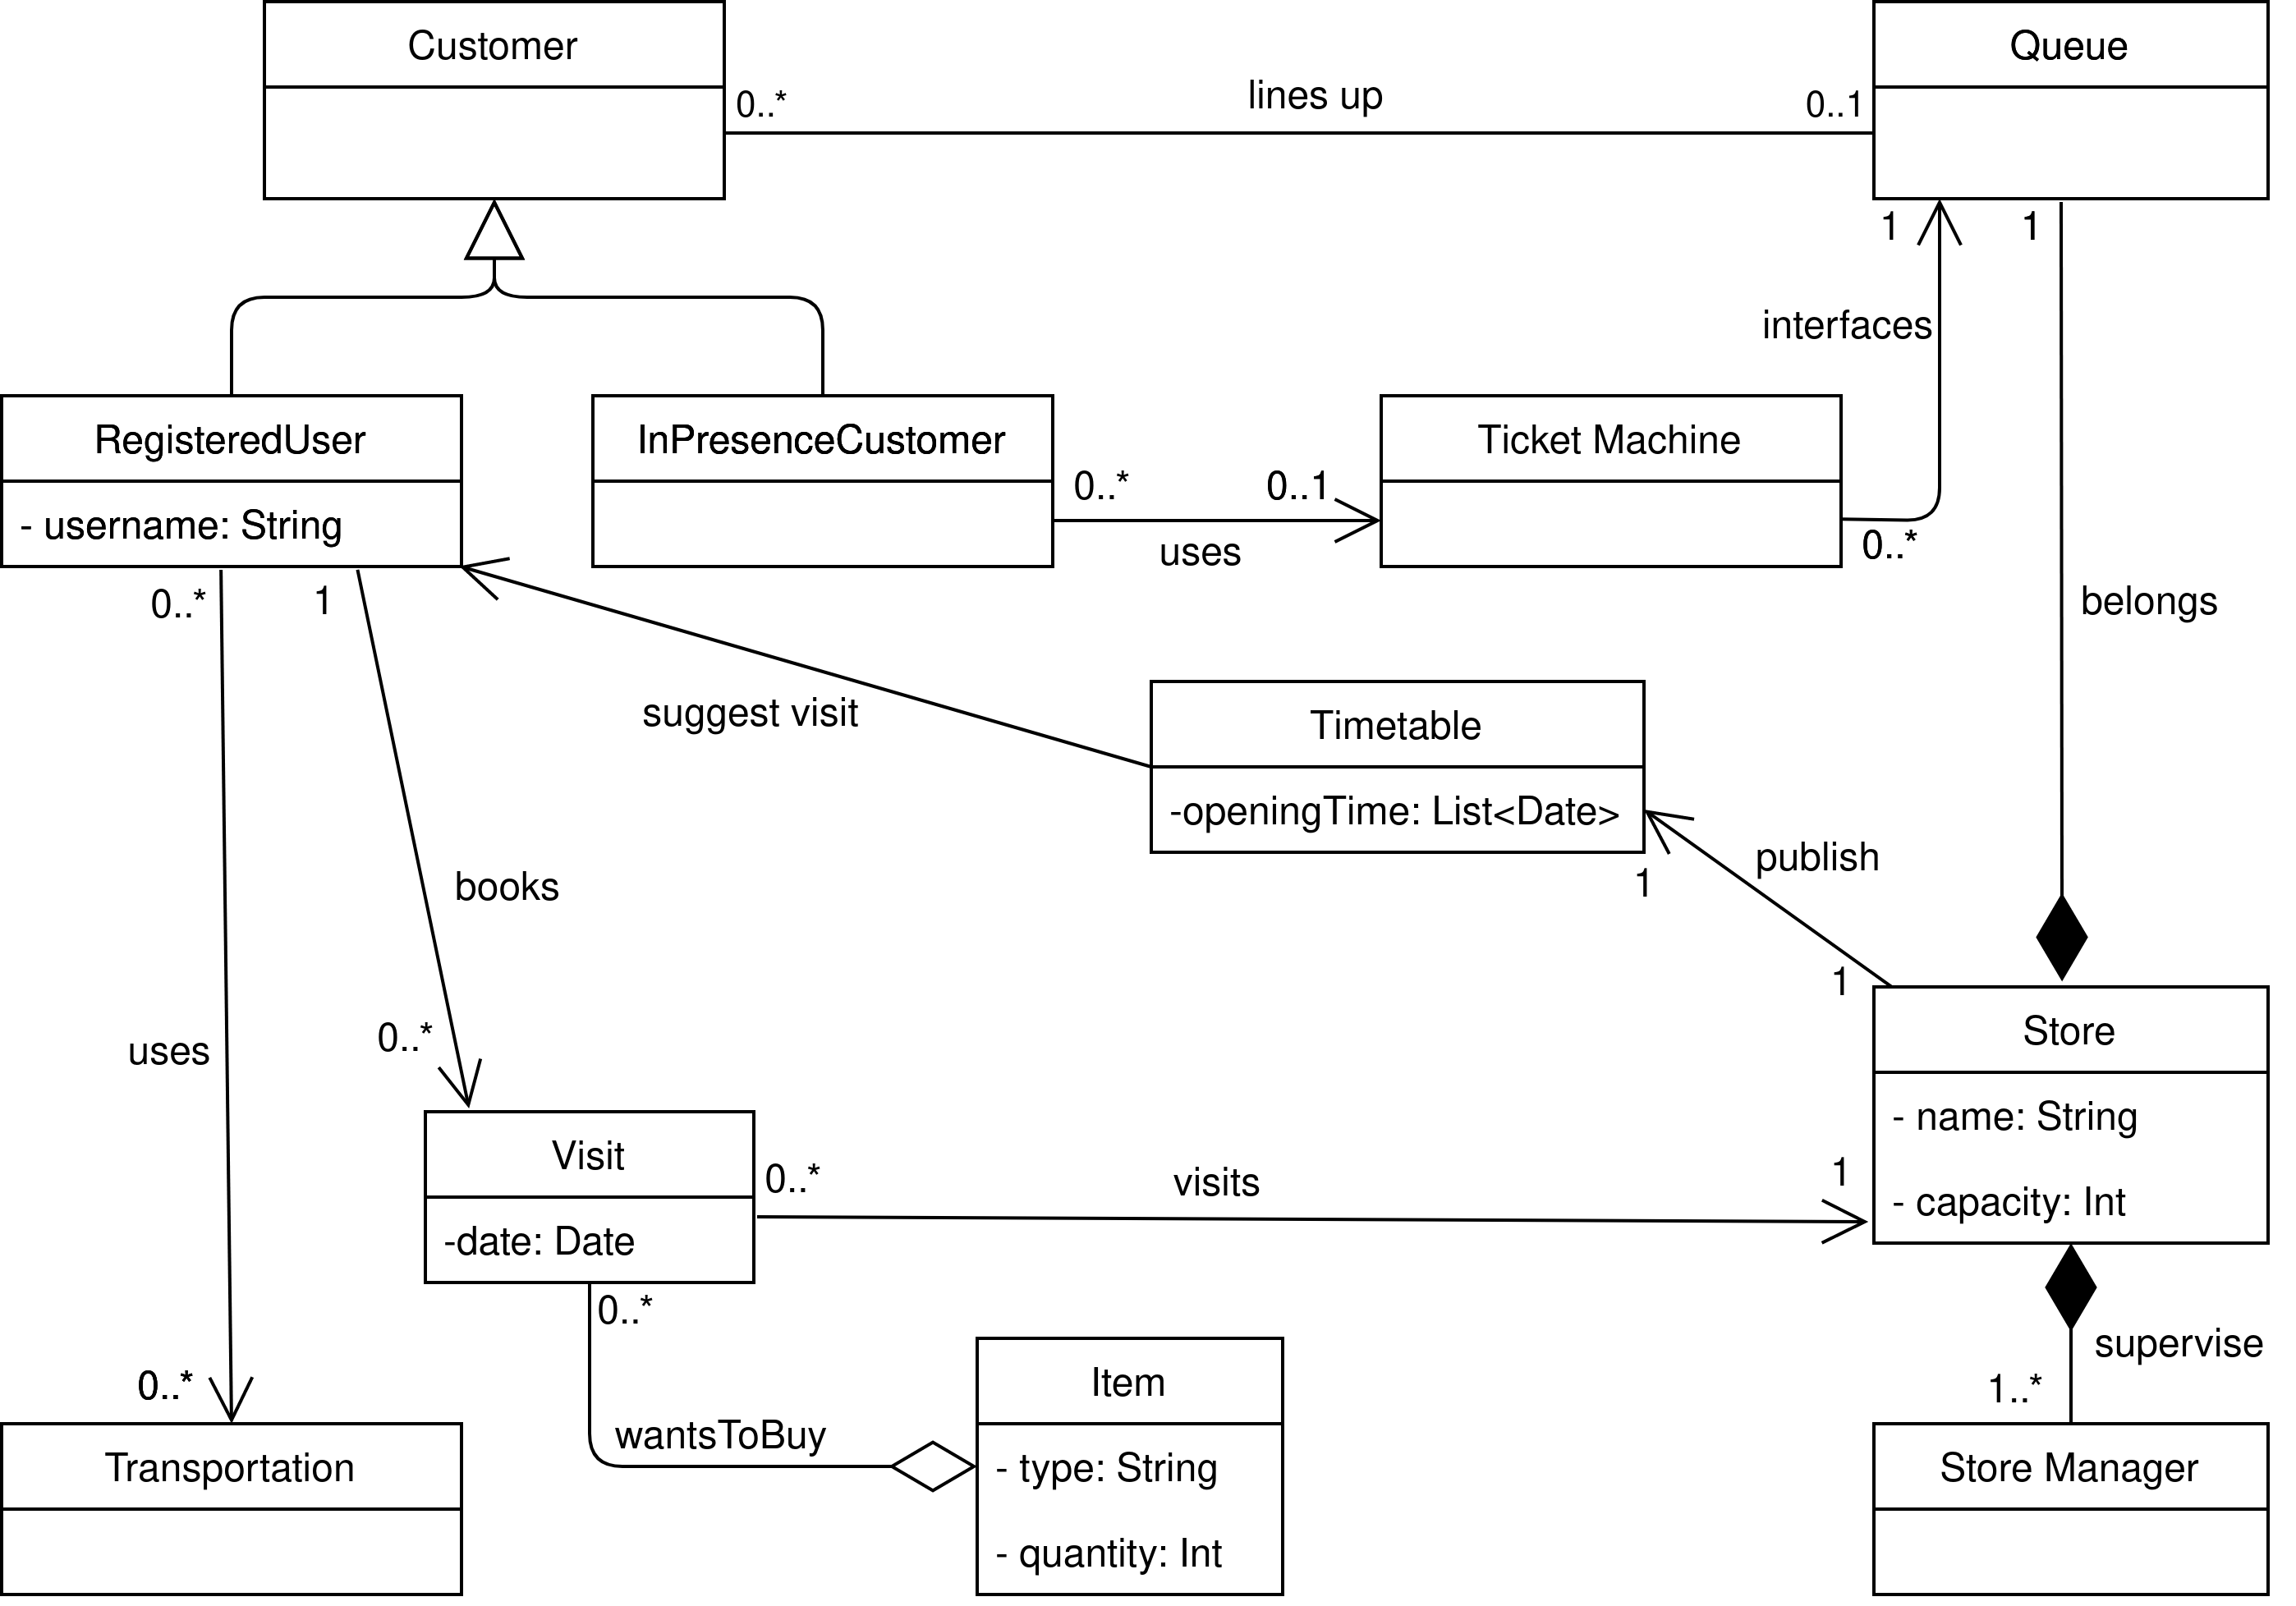
\includegraphics[scale=0.5]{UML_class_diagram.png}
			\caption{Class diagram}
			\label{fig:class_diagram}
		\end{figure}
		
	
		\subsection{StateCharts}
		In this section we want to show the evolution over time of the states of the application and the behavior of the user interacting with the app and the environment.
The state diagrams below better explain the progress of the system.

		\begin{figure}[htp]
			\centering
			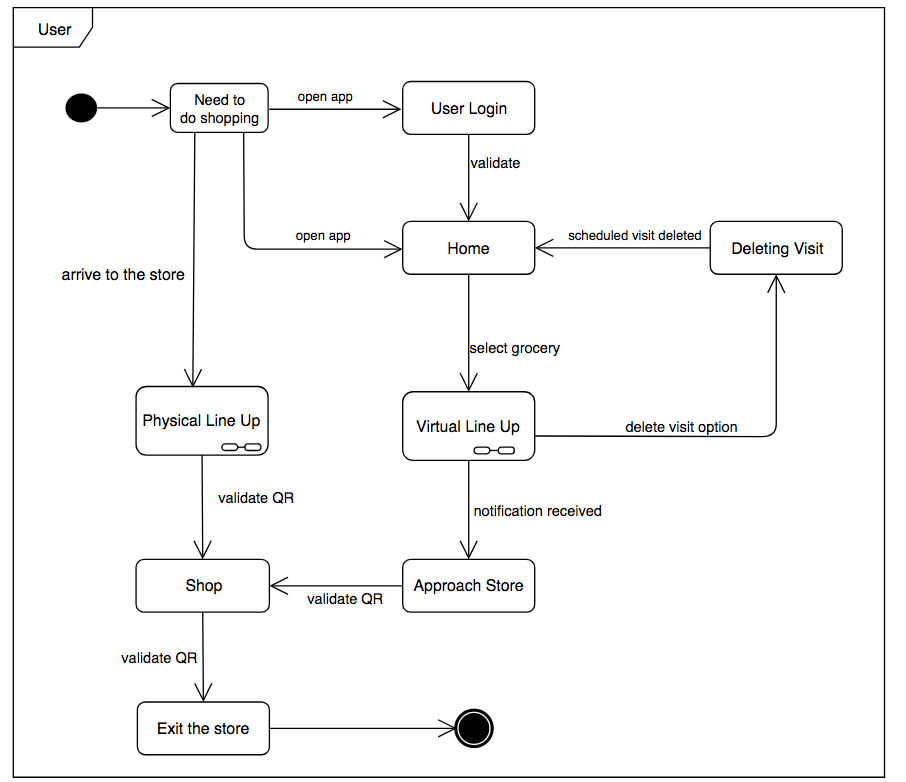
\includegraphics[scale=0.5]{user.png}
			\caption{State Diagram}
			\label{figure 1:  User}
		\end{figure}
		
		In the first state diagram (figure 1) it’s shown how the user interacts with the environment and the system when he needs to do shopping. He interacts with the system lining up to a store in a virtual way using the mobile or web application, or queuing physically at the store he wants to visit.
What’s more, to enter the store, he needs to show the QR-code, and then he has to do the same when he exits, so that the queue can proceed. 

		\begin{figure}[htp]
			\centering
			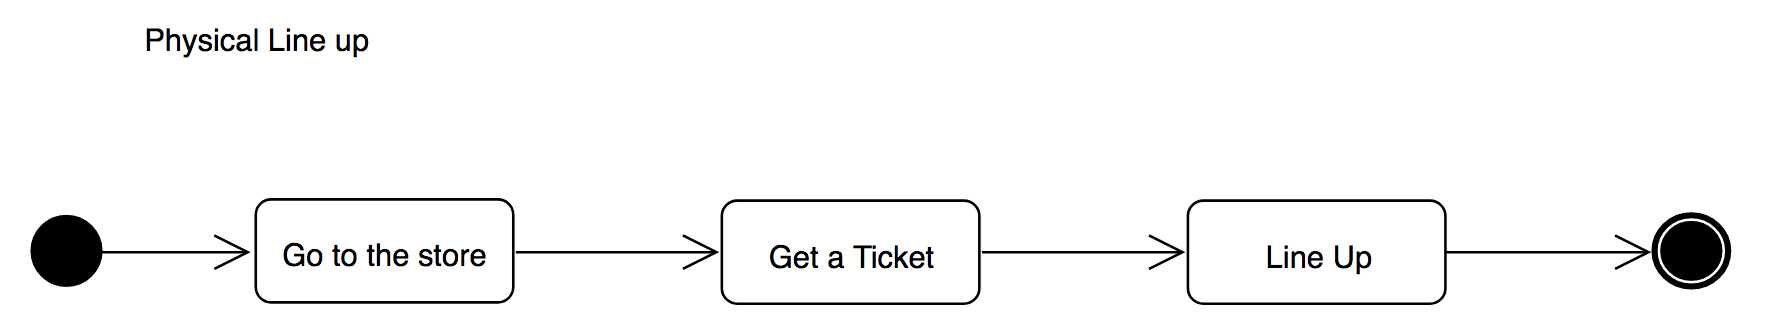
\includegraphics[width=\linewidth]{physicalqueue.png}
			\caption{State Diagram}
			\label{figure 2:  Physical Queue}
		\end{figure}
		
		In this second state diagram (figure 2) it’s better explained the physical line up of the user, that directly gets a ticket nearby the store.
		
		\begin{figure}[htp]
			\centering
			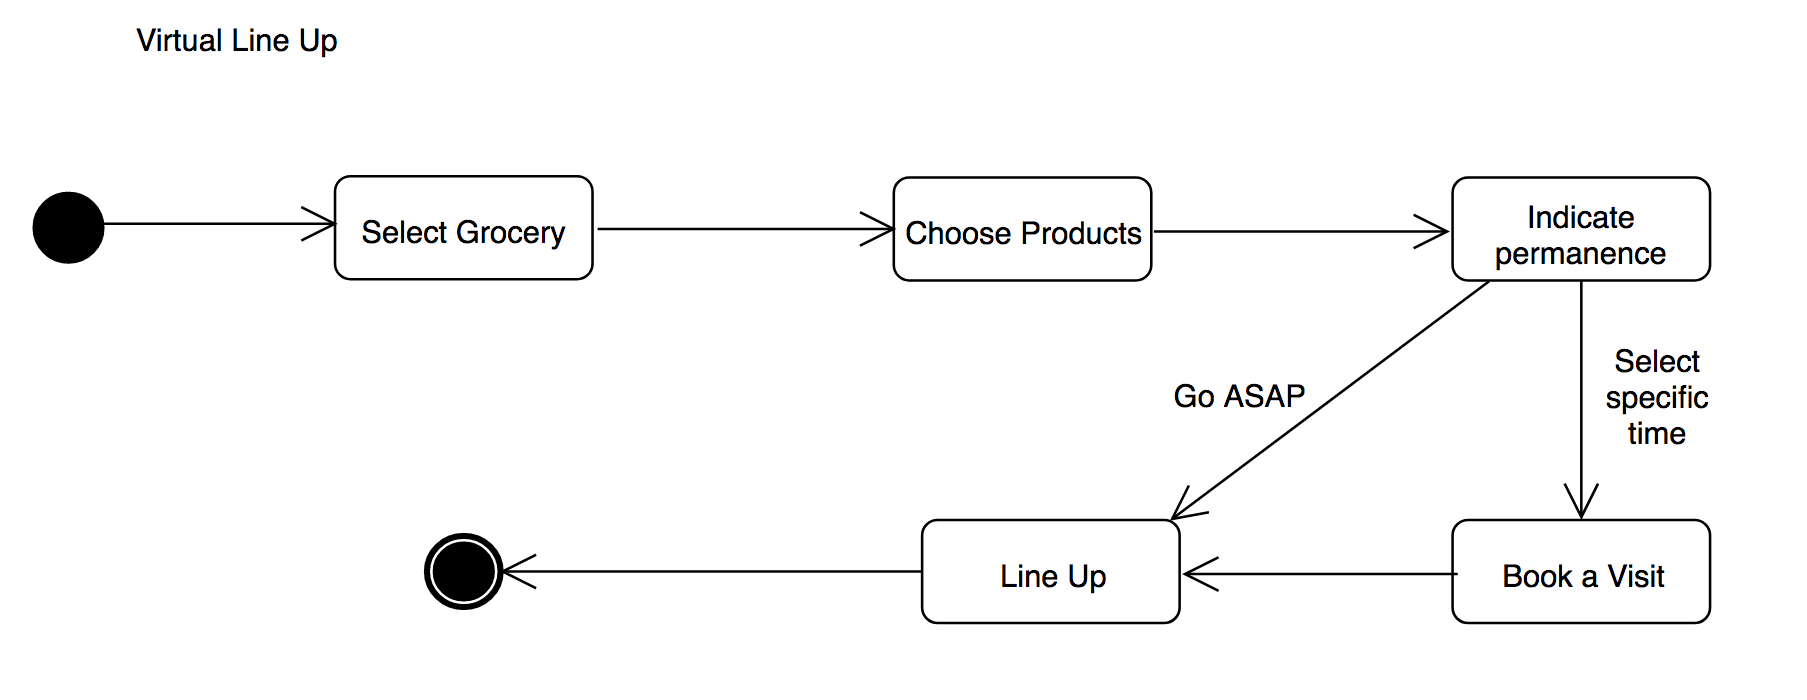
\includegraphics[width=\linewidth]{virtualqueue.png}
			\caption{State Diagram}
			\label{figure 3:  Virtual Queue}
		\end{figure}
		
		Here (figure 3) are shown the steps to go through the virtual line up of the user, that has to face some intermediate steps before he gains the possibility to line up to the store.
		
		\begin{figure}[htp]
			\centering
			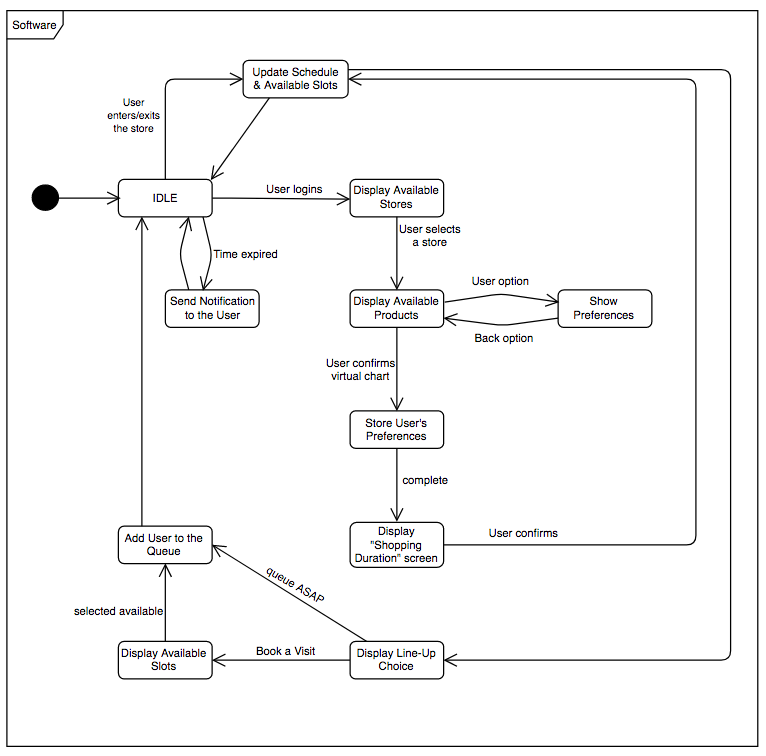
\includegraphics[width=\linewidth]{software.png}
			\caption{State Diagram}
			\label{figure 4:  Software}
		\end{figure}
		
		This fourth state chart (figure 4) shows how the system behaves when a user lines up, storing his preferences to allow to suggest the products that the user might enjoy during the next sessions, but also to update the schedule to permit to book visits into the selected store. It’s important to say that here’s explained how the system behaves with respect to a single user, but it has to concurrently work for all the users connected. 
The possibility to update the schedule is also left when the system idles, so that it can deal with eventual withdraws of the users or because some tickets are taken physically at the store and the software needs to be updated about them. In addition, it’s also shown that the system needs to notify the user to approach the store when his turn is about to come.
		
	
	\section{Specific requirements}
	\section{Formal analysis using Alloy}
	\section{Effort spent}
	\textbf{\large Riccardo Nannini:} \\ \newline
		\begin{tabular}{|l|c|}
			\hline
			Discussion on the first section &  \textbf{2h} \\ \hline
			\rowcolor[HTML]{DCDCDC} 
			World and Shared Phenomena \& Goals & \textbf{3h} \\ \hline
			Product perspective \& class diagram & \textbf{3h} \\ \hline
		\end{tabular}
	
	\section{References}				
	\end{document}
